\documentclass[final]{beamer}
\usefonttheme[onlymath]{serif}
\usepackage{subfig}
\usepackage{xcolor}
\usepackage[utf8]{inputenc}
\usetheme{SUPoster}
\usepackage{multicol}
\usepackage{diagbox}
\usepackage{tabularx}
\usepackage{booktabs}
\usepackage{todonotes}

\usepackage[orientation=landscape,size=a1,scale=1.6]{beamerposter}

\captionsetup[figure]{labelformat=empty}% redefines the caption setup of the figures environment in the beamer class.
%\captionsetup[subfigure]{labelformat=empty}
\usepackage[absolute,overlay]{textpos}
\setlength{\TPHorizModule}{1cm}
\setlength{\TPVertModule}{1cm}


\usepackage{lmodern} % needed to make math mode fonts scale properly
\usepackage{url}
\usepackage{graphics}
\usepackage{bold-extra}
\usepackage{movie15}
\usepackage{caption}

\usepackage{enumitem}
% \setitemize[1]{label=$\blacktriangleright$}
% \setlist[itemize,1]{label=$\blacktriangleright$}

\setlist[itemize]{label=\usebeamerfont*{itemize item}%
  \usebeamercolor[fg]{itemize item}
  \usebeamertemplate{itemize item},
  leftmargin=1em}

% next line is necessary to make beamer and enumitem play nicely together (see http://tex.stackexchange.com/questions/45921/make-enumerate-have-beamer-themes-when-using-enumitem/45950#45950)
\setlist[enumerate]{leftmargin=2.2em,%
label=\protect\usebeamerfont{enumerate item}%
    \protect\usebeamercolor[fg]{enumerate item}%
    \insertenumlabel. }

%% DOCUMENT DATA

\title{A Formal Methods Approach Towards Deep Learning Interpretability}

\author{Kriten Kessel, Christopher Lazarus, Javier Sagastuy}
\institute{Stanford University}

\logoleft{\begin{center} 
\includegraphics[height=4.5cm]{img/SU_Seal_Blk_pos}\end{center}}
\logoright{\begin{center} 
\includegraphics[height=4.5cm]{img/icme_logo_trans} \end{center}}
\footer{CS 236: Deep Generative Models $|$ Fall 2019 \hspace{38cm} \{\texttt{chami, clazarus, marcthib}\}\texttt{@stanford.edu} }
%\date{}

\begin{document}


\definecolor{almostWhite}{RGB}{240,240,240}
\definecolor{lightGray}{RGB}{220,220,220}
\definecolor{tbllinecolor}{RGB}{200,200,200}
\beamertemplateshadingbackground{lightGray}{almostWhite}
\newcommand{\vltbl}{{\color{tbllinecolor}\vrule}}


\begin{frame}[fragile]{}

%%%%%%%%%%%%%%%%%%%%%%%%%%%%%%%%%%%%%%%%%%%%%%%%%%%%%%%%%%%%%%%%%%%%
% IMPORTANT:
%   Here is where you define your poster's layout params (widths and
%   vertical positions).
%   Feel free to add/remove more, to make your layout fit your needs
%
%   All dimensions are in cm (I think).
%%%%%%%%%%%%%%%%%%%%%%%%%%%%%%%%%%%%%%%%%%%%%%%%%%%%%%%%%%%%%%%%%%%%

% centralize columns layout
\newcommand{\vstart}{58} % where the top row start vertically
\newcommand{\vstartCols}{8} % where the columns start vertically
\newcommand{\fullwidth}{81}  % this is the key to the values below
\newcommand{\colwidth}{26.5}

\newcommand{\firstcolpos}{1}
\newcommand{\secondcolpos}{28.75}
\newcommand{\thirdcolpos}{56.5}
\newcommand{\bottomblockstart}{108.5}


% this will add some padding to the blocks, to avoid text reaching
% the border (looks bad)
\newenvironment{paddedBlock}[2][0.95\linewidth]
    {\begin{block}{#2}\begin{minipage}{#1}}
    {\end{minipage}\end{block}}

%%%%%%%%%%%%%%%%%%%%%%%%%%%%%%%%%%%%%%%%%%%%%%%%%%%%%%%%%%%%%%%%%%%%
% And now ... the content
%%%%%%%%%%%%%%%%%%%%%%%%%%%%%%%%%%%%%%%%%%%%%%%%%%%%%%%%%%%%%%%%%%%%

%%%%%%%%%%%%%%%%%%%%%%%%%
%%%%%%%%%%%%%%%%%%%%%%%%%
%% LEFT COLUMN
%%%%%%%%%%%%%%%%%%%%%%%%%
%%%%%%%%%%%%%%%%%%%%%%%%%
\begin{textblock}{\colwidth}(\firstcolpos,\vstartCols)

\begin{paddedBlock}{Summary}
We tackle the problem of \textbf{node classification} where the goal is to classify nodes in a graph by leveraging nodes' features and graph structure.
We focus on \textbf{semi-supervised} settings where only a subset of nodes is labelled and we aim at \textbf{transferring knowledge} across labelled and unlabelled nodes. 
\begin{itemize}
\item \textbf{Problem:} node classification on a new population, not connected to the labelled nodes
\item \textbf{Solution:} hallucinate edges between the labelled nodes and the unlabelled nodes, to reinforce the information flow
\item \textbf{Results:} our method achieves +3.6\% and +3.4\% gain in accuracy over standard baselines on \texttt{cora} and \texttt{citeseer} datasets.
\end{itemize}
\end{paddedBlock}

\begin{paddedBlock}{Problem Setup}
\underline{Input}:
\begin{itemize}
\item adjacency matrices $A_L$ and $A_U$ for the two sets of nodes;
\item features vectors $X_L$ and $X_U$;
\item labels $y_L$
\end{itemize}
\begin{figure}
    \centering
    %\missingfigure[width=0.5\textwidth]{2 graphs fig}
    %\missingfigure{figure with the two graphs (one labeled and one not) goes here}
    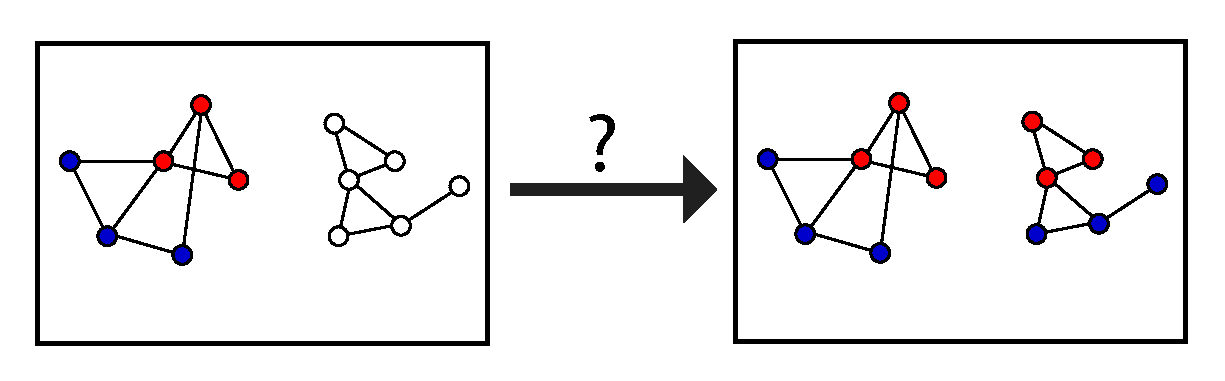
\includegraphics[width=0.90\textwidth]{img/graph_prob.pdf}
    %\caption{Caption}
    \label{fig:coins}
\end{figure}
\underline{Output}:
\begin{itemize}
	\item predictions for the unlabelled nodes $\hat{y}_L$
\end{itemize}
%\vspace{-5mm}
\end{paddedBlock}

\begin{paddedBlock}{Baseline model}
\texttt{GCN} [1] for node classification: $\hat{y} = h(Ah(AXW_1)W_2)$
\begin{figure}
    \centering
    %\missingfigure[width=0.5\textwidth]{2 graphs fig}
    %\missingfigure{architecture of the baseline model}
    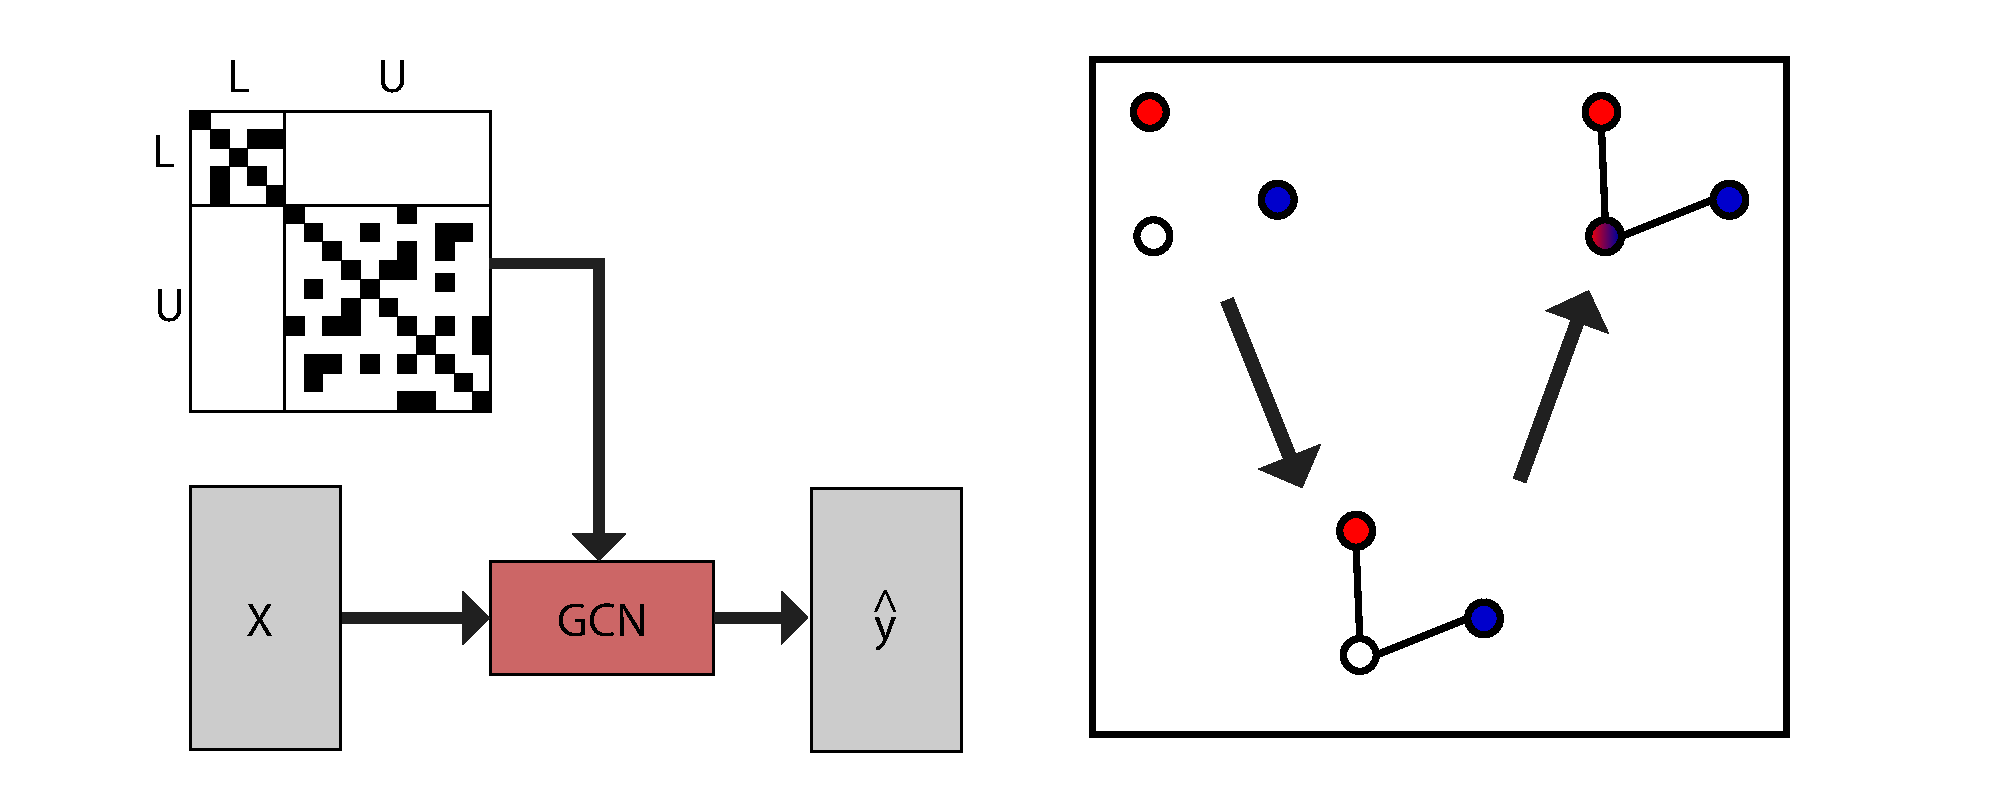
\includegraphics[width=.8\textwidth]{img/model_small.pdf}
    %\caption{Caption}
    \label{fig:small}
\end{figure}
\end{paddedBlock}
\end{textblock}

%%%%%%%%%%%%%%%%%%%%%%%%%
%%%%%%%%%%%%%%%%%%%%%%%%%
%% RIGHT COLUMN
%%%%%%%%%%%%%%%%%%%%%%%%%
%%%%%%%%%%%%%%%%%%%%%%%%%
\begin{textblock}{\colwidth}(\secondcolpos,\vstartCols)
\begin{paddedBlock}{Approach - Hallucigraph}
%\vspace{8mm}

\alert{Three-step process}
  \begin{itemize}
    \item learn low-dimensional node embeddings to encode node similarity (\texttt{VGAE} [2])
    \item hallucinate edges and complete the adjacency matrix (edges) 
    \item run a \texttt{GCN} with the completed adjacency to predict node labels
  \end{itemize}
  \begin{figure}
      \centering
      %\missingfigure[width=0.5\textwidth]{2 graphs fig}
      %\missingfigure{Fancy figure with projected graphs}
      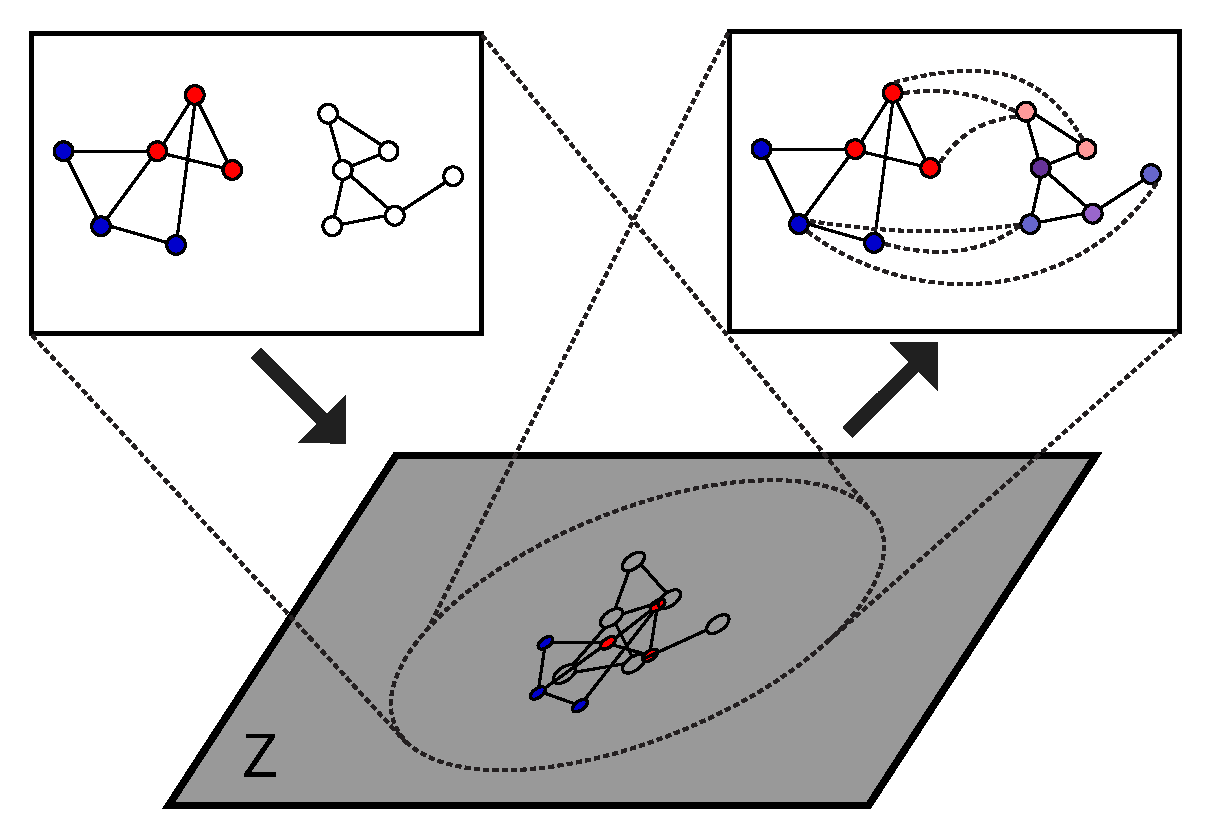
\includegraphics[width=0.60\textwidth]{img/graph_fig2.pdf}
      %\caption{Caption}
      \label{fig:coins}
  \end{figure}
%\vspace{8mm}

\alert{1. Link prediction - Variational Graph Auto-Encoder (\texttt{VGAE}):}
\begin{itemize}
  \item $Z\sim\mathcal{N}(\mu_Z,\sigma_Z^2)\ \ \mathrm{and}\ \ \tilde{A}=\sigma(ZZ^T).$
  \item with $\mu_Z,\sigma_Z=\mathrm{GCN}(A, X)$
\end{itemize}
\begin{align*}
\mathcal{L}_{LP}=&-\mathbb{E}_{Z\sim q(Z|A,X)}[A_{ij}\mathrm{log}\tilde{A}_{ij}+(1-A_{ij})\mathrm{log}(1-\tilde{A}_{i,j})]\\
&+\mathrm{KL}(q(Z|A,X)||p(Z)).
\end{align*}
%\vspace{-8mm}
\begin{figure}
    \centering
    %\missingfigure[width=0.5\textwidth]{2 graphs fig}
    %\missingfigure{Hallucigraph architecture sketch}
    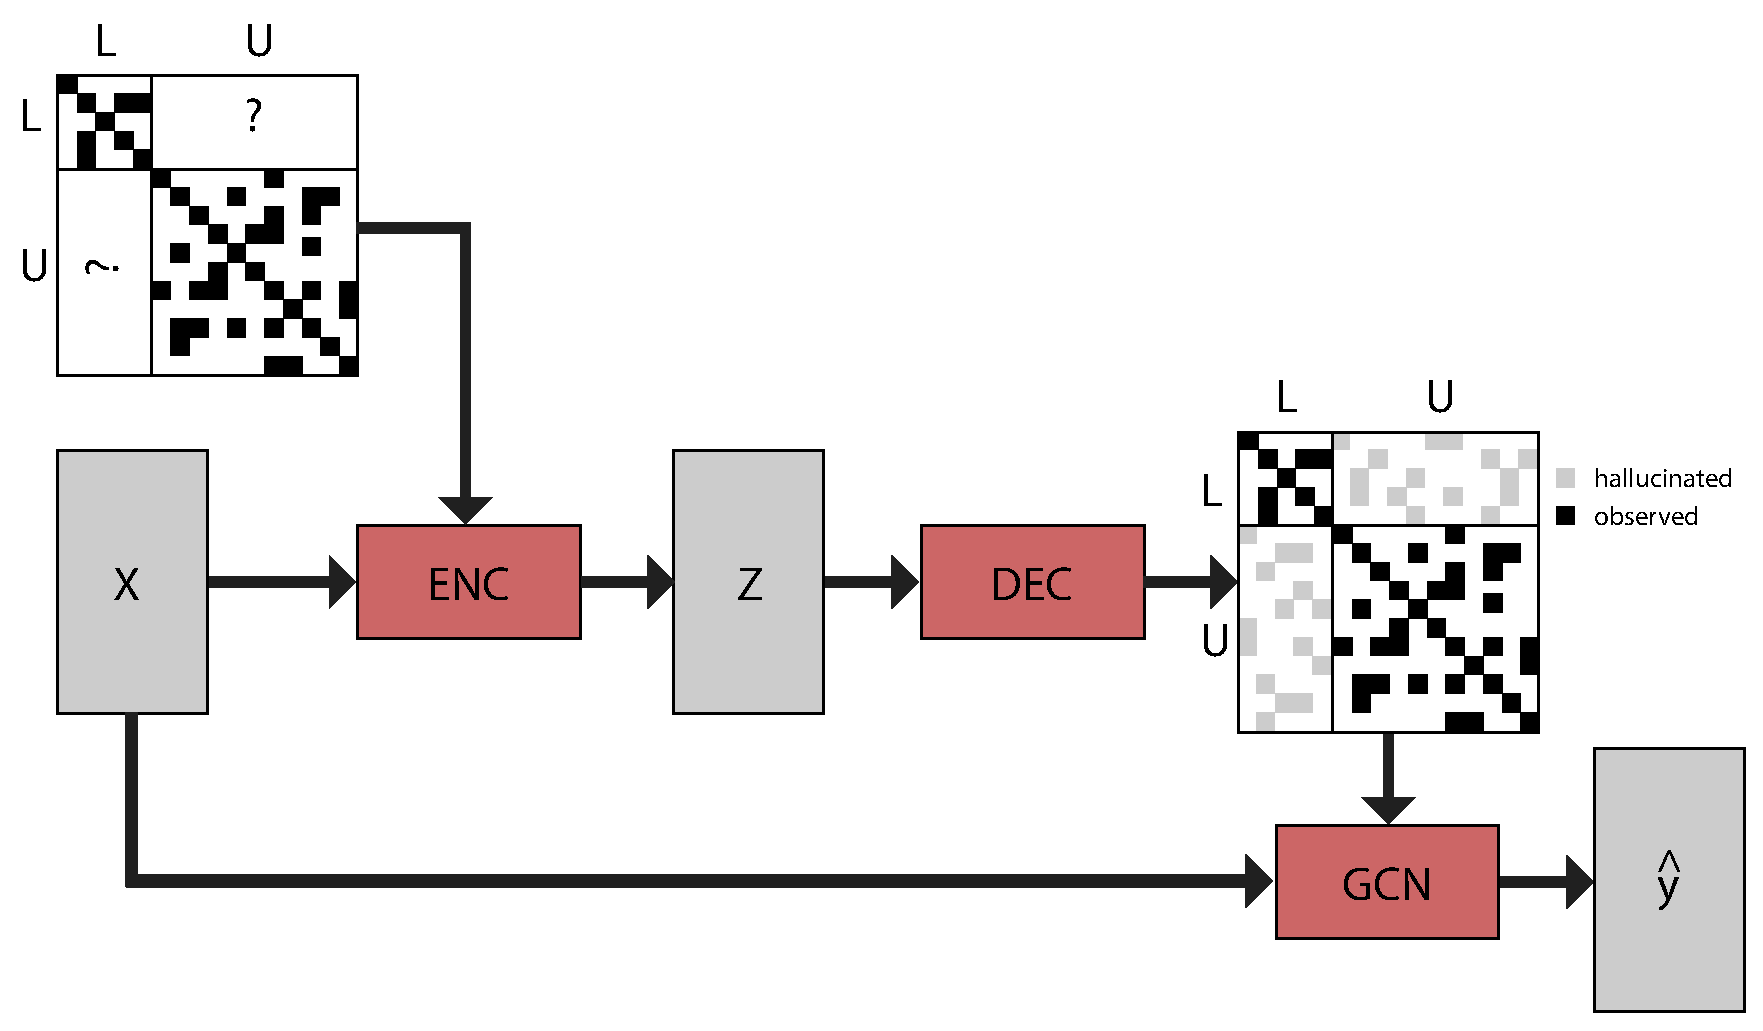
\includegraphics[width=.8\textwidth]{img/model_big.pdf}
    %\caption{Caption}
    \label{fig:big}
\end{figure}
%\vspace{8mm}
\alert{2. Edge hallucination}
  produces $\hat{A}$:
  \begin{itemize}
    \item top$K$ ($K$ hyper-parameter)
    \item sampling using gumbel softmax [4] trick (allows gradients to flow)
  \end{itemize}
\alert{3. Node classification}
\begin{itemize}
	\item $\hat{y} = \mathrm{GCN}(\hat{A}, X)$
\end{itemize}

\end{paddedBlock}
%\vspace{3mm}
\end{textblock}


\begin{textblock}{\colwidth}(\thirdcolpos,\vstartCols)

%\begin{paddedBlock}

%\
%$\hat{y}=\mathrm{GCN}(\hat{A}, X)$

%\end{paddedBlock}

\begin{paddedBlock}{Results}
%\vspace{8mm}

\alert{Classification performance per number of hallucinated edges (cora)}
  \begin{figure}
      \centering
      %\missingfigure[width=0.5\textwidth]{2 graphs fig}
      %\missingfigure{Edge inference ROC curve}
      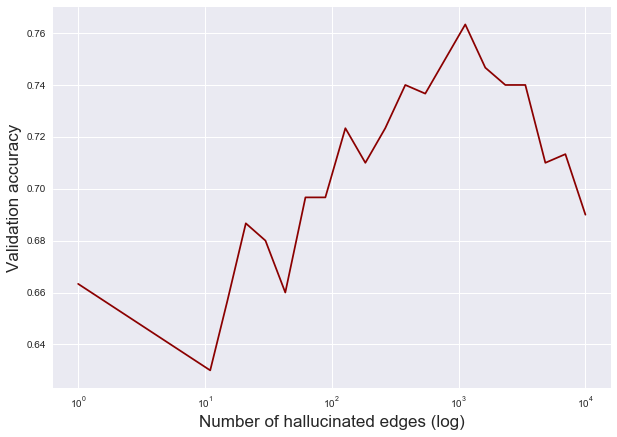
\includegraphics[width=.8\textwidth]{img/acc_vs_topk.png}
      %\caption{Caption}
      \label{fig:coins}
  \end{figure}

%\vspace{8mm}
\alert{Node classification results}

\begin{table}[h!]\centering
\begin{tabular}{@{}rr|rrcrrrcrrr@{}}\toprule
\multicolumn{1}{c}{Model} & \phantom{abc}  &\multicolumn{1}{c}{cora} & \phantom{abc}  & \multicolumn{1}{c}{citeseer}  \\
\midrule
\midrule
\multicolumn{1}{c}{MLP} & \phantom{abc}  &56.4\% &  &56.8 \%   \\
\midrule
\multicolumn{1}{c}{GCN} & \phantom{abc}  &71.3\% &  & 65.8\%   \\
\midrule
\multicolumn{1}{c}{Hallucigraph} & \phantom{abc}  &\textbf{74.9\%} &  & \textbf{69.2\%}   \\
\bottomrule
\end{tabular}
\caption{Accuracy results for node classification task on three publication datasets where we removed all $LU$ edges; using plain nodes features without edges (MLP); using the edges within labelled nodes and within unlabelled nodes (GCN); using Hallucigraph.}
\label{restable}
\end{table}

\begin{itemize}
  \item As shown in [1], the GCN improves on standalone MLP by leveraging the connections between nodes
  \item By adding "hallucinated" edges, we improve the connectivity structure, and we obtain more predictive power
\end{itemize}

\end{paddedBlock}


\begin{paddedBlock}{References}
\footnotesize{[1] Thomas N Kipf and Max Welling. Semi-supervised classification with graph convolutional
networks. arXiv preprint arXiv:1609.02907, 2016.}

\footnotesize{[2] Thomas N Kipf and Max Welling. Variational graph auto-encoders. arXiv preprint
arXiv:1611.07308, 2016.}

\footnotesize{[3] Aditya Grover, Aaron Zweig, and Stefano Ermon. Graphite: Iterative generative modeling of
graphs. arXiv preprint arXiv:1803.10459, 2018}

\footnotesize{[4] Eric Jang, Shixiang Gu, and Ben Poole. Categorical reparameterization with gumbel-softmax.arXiv preprint arXiv:1611.01144, 2016}

\end{paddedBlock}
\end{textblock}


%%%%%%%%%%%%%%%%%%%%%%%%%
%%%%%%%%%%%%%%%%%%%%%%%%%
%% BOTTOM ROW
%%%%%%%%%%%%%%%%%%%%%%%%%
%%%%%%%%%%%%%%%%%%%%%%%%%

%\begin{textblock}{\fullwidth}(2,\bottomblockstart)
%\begin{paddedBlock}[0.98\linewidth]{Acknowledgements}

%In case you need it, you can do this too

%\end{paddedBlock}
%\end{textblock}

\end{frame}
\end{document}
